\documentclass[aspectratio=169]{beamer}
\setbeamertemplate{navigation symbols}{}
\usepackage{color, amsmath, comment, subfigure}
\usepackage{url}

\usepackage{hyperref}
\hypersetup{
    colorlinks=true,
    linkcolor=blue,
    filecolor=magenta,      
    urlcolor=cyan,
}

%%%%%%%%%%%%%%%%%%%%%%%%%%
\title[]{Comments slides for Tuesday, Sept 29:\\Online ads}
\author[]{Matthew J. Salganik}
\institute[]{}
\date[]{COS 597E/SOC 555 Limits to prediction\\Fall 2020, Princeton University}

\begin{document}
%%%%%%%%%%%%%%%%%%%%%%%%%%%
\frame{\titlepage}
%%%%%%%%%%%%%%%%%%%%%%%%%%%
\begin{frame}
\frametitle{}

Observations/comments/questions/provocations:
\begin{itemize}
\item The readings about the complexity of measuring the effectiveness of ads is consistent with my experience.  This is hard.
\pause
\item Beware of estimates in fields where people are strongly incentivized to get a certain result. But sometimes this can leave fingerprints . . . . 
\end{itemize}

\end{frame}
%%%%%%%%%%%%%%%%%%%%%%%%%%%
\begin{frame}
\frametitle{}

\begin{center}
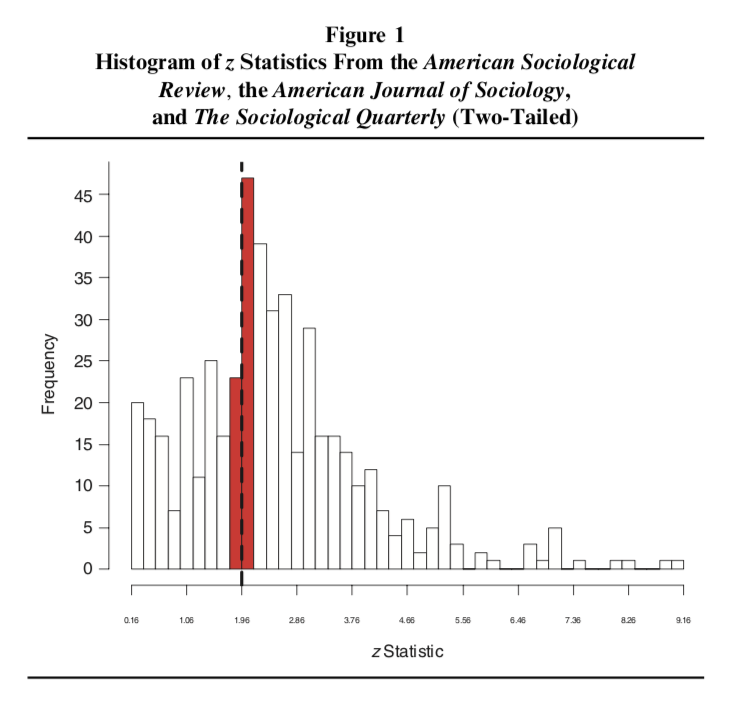
\includegraphics[width=0.5\textwidth]{figures/gerber_publication_2008_fig1}
\end{center}

\vfill
Are there fingerprints like this in the $\hat{y}$ world? Is it caused by researchers or journals?\\
Figure is from \href{https://doi.org/10.1177/0049124108318973}{Gerber and Malhotra (2008)}
\end{frame}
%%%%%%%%%%%%%%%%%%%%%%%%%%
\begin{frame}
\frametitle{}

Observations/comments/questions/provocations:
\begin{itemize}
\item The readings about the complexity of measuring the effectiveness of ads is consistent with my experience.  This is hard.
\item Beware of estimates in fields where people are strongly incentivized to get a certain result. But sometimes this can leave fingerprints . . . . 
\item In the case of ads, the predictor also partially controls the data generating process (compare to weather for example). How is that leveraged? How could it be?
\pause
\item The observed ad click rates is not a good measure of the maximum possible click rate.
\pause
\item It is hard for anyone outside ad serving companies to know the accuracy of click predictions.
\pause
\item There are still real computational issues.
\pause
\item They calculate AucLoss (1 - AUC), LogLoss, and SquaredError. Why not \$? How should we balance between three metrics?
\pause
\item ``Absolute metrics are misleading'' They look at relative performance (\% change relative to a benchmark model on exactly the same data). How many papers have we read with absolute measures (e.g., ImageNet)? When are absolute measures better? When relative? When do we only care about the order?
\end{itemize}

\end{frame}
%%%%%%%%%%%%%%%%%%%%%%%%%%%
\begin{frame}
\frametitle{}

\begin{center}
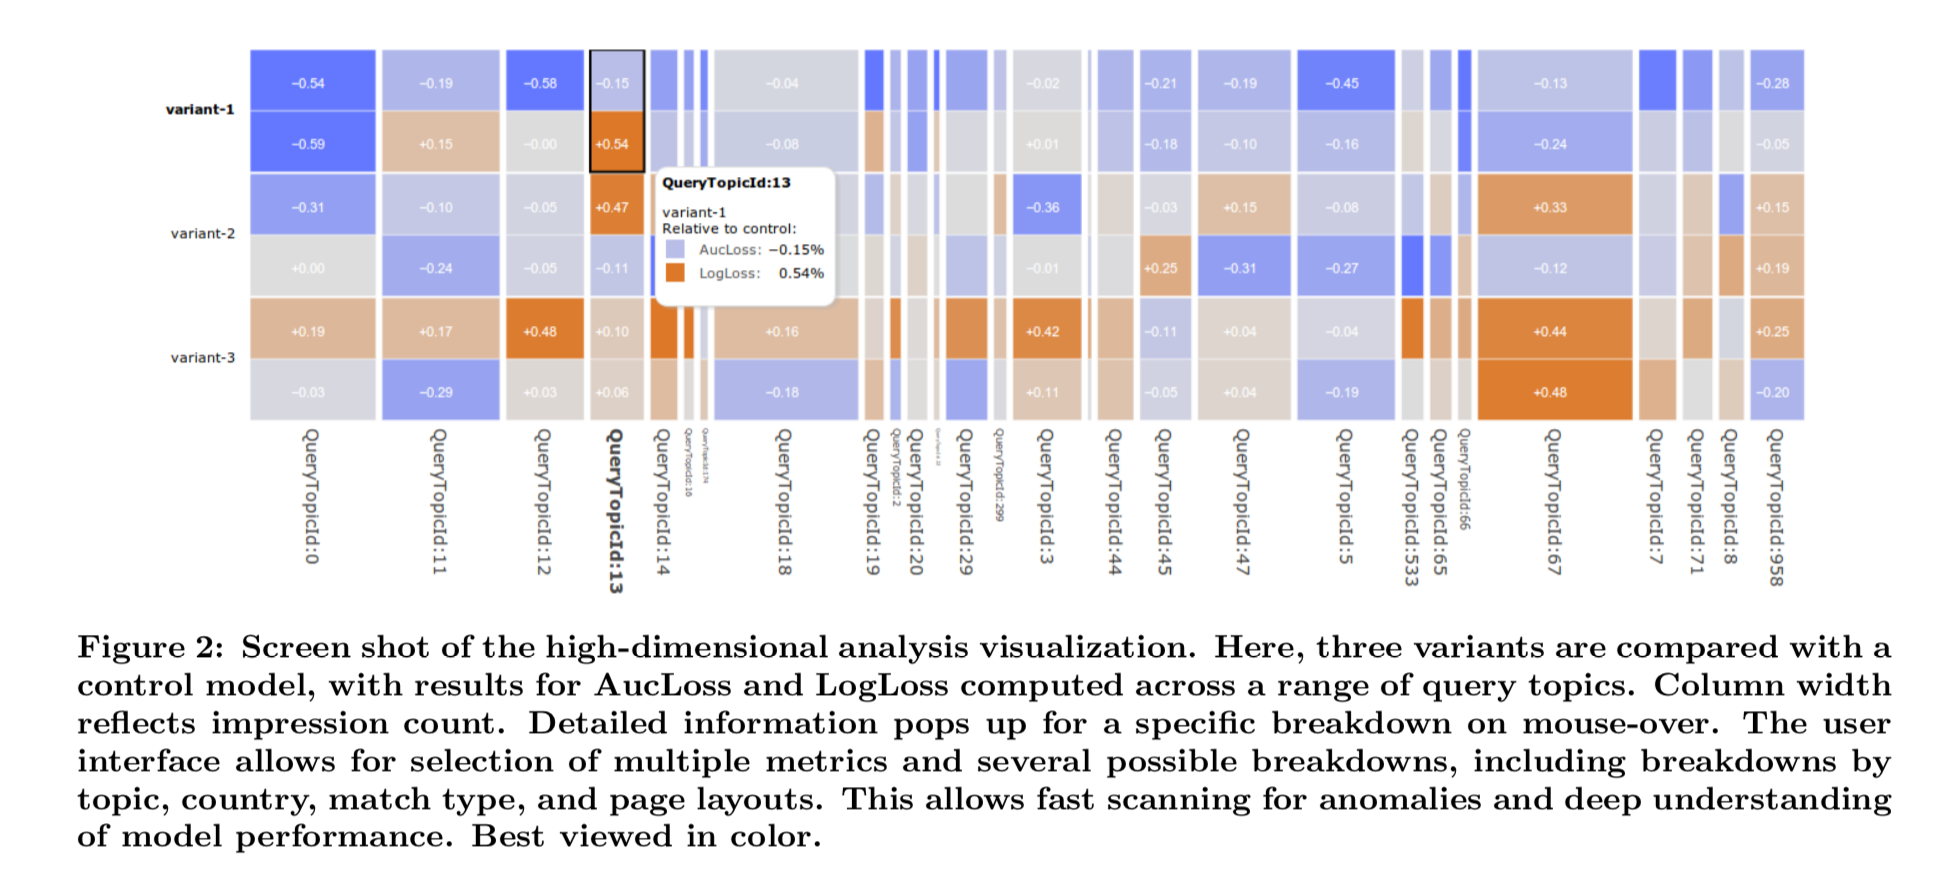
\includegraphics[width=0.9\textwidth]{figures/mcmahan_ad_2013_fig2}
\end{center}

\vfill
Heterogeneity builds insight
\end{frame}
%%%%%%%%%%%%%%%%%%%%%%%%%%




\frame{\titlepage}


\end{document}
